\documentclass[a4paper,twoside]{article}
%DIF LATEXDIFF DIFFERENCE FILE
%DIF DEL /home/resort/Documents/repos/StoryProjectionOnto/paper/icaart2027_revised/build/submitted_flat.tex   Fri Nov 13 20:13:26 2026
%DIF ADD /home/resort/Documents/repos/StoryProjectionOnto/paper/icaart2027_revised/build/revised_flat.tex     Fri Nov 13 20:13:26 2026
\usepackage[T1]{fontenc}
\usepackage[utf8]{inputenc}
\usepackage{epsfig}
\usepackage{subcaption}
\usepackage{calc}
\usepackage{amssymb}
\usepackage{amstext}
\usepackage{amsmath}
\usepackage{amsthm}
\usepackage{multicol}
\usepackage{pslatex}
\usepackage{apalike}
\usepackage{algorithm2e}
\usepackage[bottom]{footmisc}
\usepackage{booktabs}
\usepackage{url}
\usepackage[hidelinks,pdfauthor={},pdftitle={Contextual Ontology Extraction and Inspection of Temporal Narrative Networks},pdfcreator={LaTeX},pdfsubject={Anonymous position paper}]{hyperref}
\usepackage{SCITEPRESS}
\newcommand{\Temperature}{0.7}
\newcommand{\TopP}{0.8}
\newcommand{\TopK}{20}
\newcommand{\Seed}{1988649846}
\newcommand{\OutputTokens}{2,048}
\newcommand{\ContextTokens}{12,288}
\newcommand{\StorySentences}{14}
\newcommand{\FableWords}{133}
\newcommand{\AliceWords}{112}
\newcommand{\HolmesWords}{159}
\newcommand{\CompactCalls}{12}
\newcommand{\ProseCalls}{9}
\newcommand{\ProseParsed}{7}
\newcommand{\IntervalsKept}{79}
\newcommand{\IntervalsEligible}{79}
\newcommand{\OrchardLocationRecall}{0.750}
\newcommand{\MainCalls}{21}
\newcommand{\MainAllocation}{454.82}
\newcommand{\CompactAllocation}{249.45}
\newcommand{\ProseAllocation}{205.37}
\newcommand{\CompactRequest}{104.72}
\newcommand{\ProseRequest}{57.24}
\newcommand{\FableAFone}{0.625}
\newcommand{\FableACoverage}{6 of 8}
\newcommand{\FableBFone}{0.308}
\newcommand{\FableBCoverage}{4 of 8}
\newcommand{\AliceAFone}{0.000}
\newcommand{\AliceACoverage}{1 of 4}
\newcommand{\AliceBFone}{0.000}
\newcommand{\AliceBCoverage}{3 of 4}
\newcommand{\FableQuestion}{Which physical running/waking, capture, binding, rope-gnawing and release relationships involve the Lion, Mouse, hunters and ropes? Exclude dialogue, intentions, laughter and the moral.}
\newcommand{\HarborQuestion}{Which directly narrated location relationships have an explicitly stated interval overlapping day 2 up to but not including day 4? Return all of them with their full evidence-stated intervals, not clipped to the question window. Exclude undated locations and beliefs.}
\newcommand{\OrchardQuestion}{Who owns or carries what? Return all and only directly narrated ownership and carrying relationships, retaining every stated interval.}
\newcommand{\OrchardBeliefQuestion}{Who explicitly believes what, and what reality is separately narrated about those same objects? Return each underlying believed relationship with its attribution and each matching narrated reality without attribution. Omit unrelated facts.}
\newcommand{\AliceActionQuestion}{Which sitting/location, reading/inspection and running relationships involve Alice, her sister, the book, bank and Rabbit? Exclude thoughts, feelings, appearance and book-content properties.}
\newcommand{\AliceClaimQuestion}{What does the passage say about the book's absent content and Alice's thoughts about the usefulness of such books and making a daisy-chain? Exclude physical actions, locations, appearance and the Rabbit; preserve questions and consideration without treating them as decisions.}
%DIF PREAMBLE EXTENSION ADDED BY LATEXDIFF
%DIF UNDERLINE PREAMBLE %DIF PREAMBLE
\RequirePackage[normalem]{ulem} %DIF PREAMBLE
\RequirePackage{color}\definecolor{RED}{rgb}{1,0,0}\definecolor{BLUE}{rgb}{0,0,1} %DIF PREAMBLE
\providecommand{\DIFaddtex}[1]{{\protect\color{blue}\uwave{#1}}} %DIF PREAMBLE
\providecommand{\DIFdeltex}[1]{{\protect\color{red}\sout{#1}}}                      %DIF PREAMBLE
%DIF SAFE PREAMBLE %DIF PREAMBLE
\providecommand{\DIFaddbegin}{} %DIF PREAMBLE
\providecommand{\DIFaddend}{} %DIF PREAMBLE
\providecommand{\DIFdelbegin}{} %DIF PREAMBLE
\providecommand{\DIFdelend}{} %DIF PREAMBLE
\providecommand{\DIFmodbegin}{} %DIF PREAMBLE
\providecommand{\DIFmodend}{} %DIF PREAMBLE
%DIF FLOATSAFE PREAMBLE %DIF PREAMBLE
\providecommand{\DIFaddFL}[1]{\DIFadd{#1}} %DIF PREAMBLE
\providecommand{\DIFdelFL}[1]{\DIFdel{#1}} %DIF PREAMBLE
\providecommand{\DIFaddbeginFL}{} %DIF PREAMBLE
\providecommand{\DIFaddendFL}{} %DIF PREAMBLE
\providecommand{\DIFdelbeginFL}{} %DIF PREAMBLE
\providecommand{\DIFdelendFL}{} %DIF PREAMBLE
%DIF HYPERREF PREAMBLE %DIF PREAMBLE
\providecommand{\DIFadd}[1]{\texorpdfstring{\DIFaddtex{#1}}{#1}} %DIF PREAMBLE
\providecommand{\DIFdel}[1]{\texorpdfstring{\DIFdeltex{#1}}{}} %DIF PREAMBLE
%DIF LISTINGS PREAMBLE %DIF PREAMBLE
\RequirePackage{listings} %DIF PREAMBLE
\RequirePackage{color} %DIF PREAMBLE
\lstdefinelanguage{DIFcode}{ %DIF PREAMBLE
%DIF DIFCODE_UNDERLINE %DIF PREAMBLE
  moredelim=[il][\color{red}\sout]{\%DIF\ <\ }, %DIF PREAMBLE
  moredelim=[il][\color{blue}\uwave]{\%DIF\ >\ } %DIF PREAMBLE
} %DIF PREAMBLE
\lstdefinestyle{DIFverbatimstyle}{ %DIF PREAMBLE
	language=DIFcode, %DIF PREAMBLE
	basicstyle=\ttfamily, %DIF PREAMBLE
	columns=fullflexible, %DIF PREAMBLE
	keepspaces=true %DIF PREAMBLE
} %DIF PREAMBLE
\lstnewenvironment{DIFverbatim}{\lstset{style=DIFverbatimstyle}}{} %DIF PREAMBLE
\lstnewenvironment{DIFverbatim*}{\lstset{style=DIFverbatimstyle,showspaces=true}}{} %DIF PREAMBLE
%DIF END PREAMBLE EXTENSION ADDED BY LATEXDIFF

\begin{document}
\title{Contextual Ontology Extraction and Inspection of Temporal Narrative Networks}
\author{}
\keywords{Natural Language Processing, Knowledge Representation and Reasoning, Large Language Models, Visualization.}
\abstract{We present a narrative extraction workflow connecting readers' questions, generated relationships, temporal and attribution details, and visual inspection of evidence and errors. We compare extraction before seeing a question followed by fixed selection with independent contextual extraction on three synthetic stories and three short published passages. Assessment separates strict agreement with reference answers from preserved meaning, relevance and unresolved interpretation. All \CompactCalls\ story responses were parseable. Fixed selection matched every possession and dated location target without extras, whereas contextual answers retained irrelevant facts. On fable actions, strict F1 was \FableAFone\ for selection and \FableBFone\ for contextual extraction. Query-guided extraction of statements and thoughts from an excerpt of Alice’s Adventures in Wonderland preserved \AliceBCoverage\ semantic targets despite zero strict F1. Prose parsing succeeded in \ProseParsed\ of \ProseCalls\ calls. The workflow makes these mixed results  easy to inspect, including useful thought representations, incorrect participants and lost conditional scope. These small development comparisons identify concrete extraction and selection problems for further research. }
\onecolumn\maketitle\normalsize\setcounter{footnote}{0}\vfill
\noindent{\small\textcolor{blue}{Blue underlined text is added.} \textcolor{red}{Red struck text is removed.} Title and abstract are unchanged. Figures are reduced here to fit deleted captions; full-size Figure 1 before/after pages follow.}\par\medskip

\section{INTRODUCTION}
\noindent Stories describe people, places and objects whose relationships change over time. Readers may \DIFdelbegin \DIFdel{want to know }\DIFdelend \DIFaddbegin \DIFadd{ask }\DIFaddend who carries an object, where it is, or what a character believes about it. \DIFdelbegin \DIFdel{We present a workflow for exploring narrative ontologies, structured representations of a story 's }\DIFdelend \DIFaddbegin \DIFadd{A comprehensive graph can obscure an answer; extracting only for a question can omit needed facts. Our workflow explores narrative ontologies: local vocabularies and records of story }\DIFaddend entities and relationships\DIFdelbegin \DIFdel{, as temporal networks. Nodes represent characters, objects or places, and edges show their relationships }\DIFdelend . \DIFdelbegin \DIFdel{Temporal details indicate when a relationship holds, while links to the text let readers check its basis. Readers can also examine whether a relationship reflects a character's belief or the narrator's account}\DIFdelend \DIFaddbegin \DIFadd{A temporal ontology also represents when relationships hold; here, intervals qualify the records. The network displays entities as nodes and relationships as edges. Source links distinguish beliefs from narration. This is a compact representation, not a complete formal theory of the story}\DIFaddend .

We compare two ways to produce a network for a reader's question. \emph{Pre-extract/select} (A) first extracts relationships without seeing the question, then selects existing records using fixed filters. \emph{Contextual extraction} (B) extracts relationships directly from the same text with the question supplied. Both use records with entity names, evidence citations, time intervals and attribution. Our contributions are:

\begin{enumerate}
\item An implemented workflow connecting narrative questions, temporal networks and source evidence. Linked views let readers inspect relationships and trace their meaning to the text (Section~3 and Figures~\ref{fig:orchard}-\ref{fig:alice}).
\item An empirical comparison of extraction before and after the question is supplied. Results on synthetic stories and published prose help distinguish problems in extracting relationships from problems in selecting relevant ones (Section~5).
\item An assessment combining agreement with reference answers, preservation of meaning, relevance and unresolved interpretation. Tables~\ref{tab:compact} and~\ref{tab:prose} and the annotated networks show useful partial results alongside errors.
\end{enumerate}

\DIFdelbegin \DIFdel{Together, these contributions support the inspection of narrative ontologies beyond a single accuracy score. Small development comparisons show which relationships survive extraction , which details are lost, and how questions affect the resulting networks}\DIFdelend \DIFaddbegin \DIFadd{This is an exploratory implementation and comparison, not a new extraction algorithm. Section~2 relates it to existing work; Section~3 explains the records and two approaches; Sections~4--5 describe evaluation and results; Sections~6--7 discuss limitations and next steps}\DIFaddend .

\begin{figure*}[!t]
\centering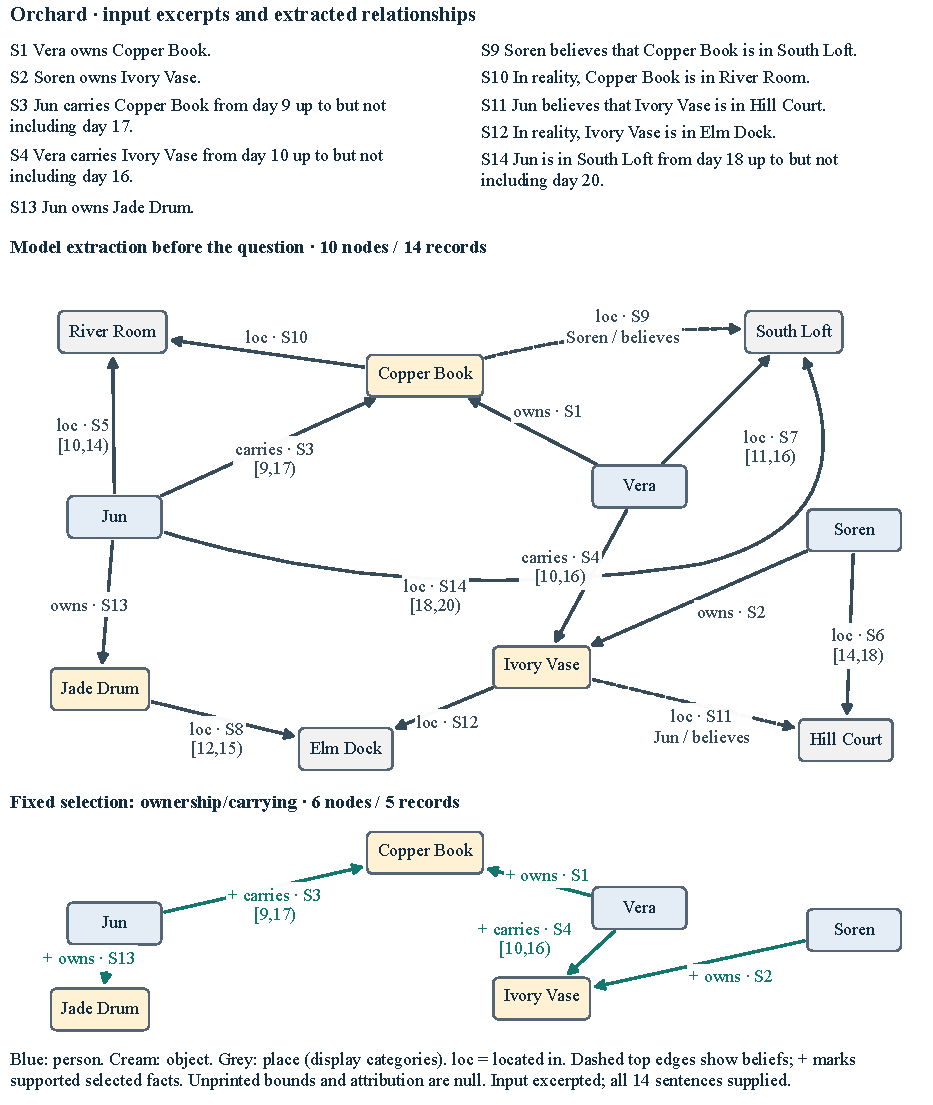
\includegraphics[width=\textwidth,height=.55\textheight,keepaspectratio]{figures/orchard_network.pdf}
\caption{Orchard \DIFdelbeginFL \DIFdelFL{: the actual }\DIFdelendFL \DIFaddbeginFL \DIFaddFL{input excerpts, }\DIFaddendFL model extraction \DIFdelbeginFL \DIFdelFL{before the question }\DIFdelendFL (top network) \DIFdelbeginFL \DIFdelFL{, followed by }\DIFdelendFL \DIFaddbeginFL \DIFaddFL{and }\DIFaddendFL fixed \DIFaddbeginFL \DIFaddFL{ownership/carrying }\DIFaddendFL selection \DIFdelbeginFL \DIFdelFL{from that extraction }\DIFdelendFL (bottom). \DIFdelbeginFL \DIFdelFL{Executed question: Who owns or carries what? Return all and only directly narrated ownership and carrying relationships, retaining every stated interval.\ All 14 extracted records and all five selected records are shown. Source excerpts S1, S3 and S11 come from the complete fourteen-sentence input. Exact endpoint strings share nodes. The selected six-node network is connected. Holder/attitude badges }\DIFdelendFL \DIFaddbeginFL \DIFaddFL{Believer names }\DIFaddendFL qualify \DIFdelbeginFL \DIFdelFL{two location }\DIFdelendFL edges\DIFdelbeginFL \DIFdelFL{without adding relationships. The broad extraction is not a gold graph. + denotes retained support for the selected records, }\DIFdelendFL \DIFaddbeginFL \DIFaddFL{; they do }\DIFaddendFL not \DIFdelbeginFL \DIFdelFL{a selection colour. Node categories are display annotations. Horizontal anchors are shared, with compressed vertical spacing below}\DIFdelendFL \DIFaddbeginFL \DIFaddFL{add relationships}\DIFaddendFL .}
\label{fig:orchard}
\end{figure*}
\section{RELATED WORK}
\noindent \emph{Extraction and representation.} TextRunner \DIFdelbegin \DIFdel{extracts relationships }\DIFdelend \DIFaddbegin \DIFadd{is an early example of extraction }\DIFaddend without a predefined relation vocabulary \DIFdelbegin \DIFdel{and indexes them for later queries }\DIFdelend \cite{banko2007}\DIFaddbegin \DIFadd{, not our experimental baseline. ReVerb constrains relation phrases }\cite{fader2011}\DIFadd{; OLLIE also retains attribution and conditional context }\cite{mausam2012}\DIFaddend . SPIRES uses recursive \DIFdelbegin \DIFdel{language model }\DIFdelend \DIFaddbegin \DIFadd{LLM }\DIFaddend prompts to fill a supplied schema and link entities to \DIFdelbegin \DIFdel{external }\DIFdelend vocabularies \cite{caufield2024}. \DIFdelbegin \DIFdel{Building on these approaches, we compare extraction with and without an available question while retaining local entity names and supporting text}\DIFdelend \DIFaddbegin \DIFadd{We compare question timing with one LLM, not these systems' extraction accuracy}\DIFaddend .

Temporal ontologies provide a foundation for describing change. OWL-Time represents instants, intervals, durations and ordering \cite{time2017}. GRaSP connects statements, textual mentions, sources and attitudes, with an interface linking events to their evidence \cite{fokkens2017}. These foundations inform our compact representation of when relationships hold and who expresses a belief.

\DIFaddbegin \DIFadd{ATOM builds and updates temporal knowledge graphs from small facts, distinguishing observation time from validity time }\cite{lairgi2026}\DIFadd{. We instead compare question-guided extraction with fixed selection; we do not test graph updating or establish an advantage over ATOM.
}

\DIFaddend \emph{Comparison and inspection.} RelVis combines extraction comparison, visual inspection and error annotation \cite{schneider2017}. It also distinguishes valid relationships missing from reference annotations from extraction errors. CaRB improves reference annotations and scoring through partial coverage and checks on the alignment of relationships and their participants \cite{bhardwaj2019}. Using our own strict matcher, we report agreement separately from judgments about preserved meaning, missing details and unresolved readings.

Our visualization draws on established filtering, linked selection and coordinated views \cite{heer2012}. \DIFdelbegin \DIFdel{The contribution brings these ideas together for narrative questions, preserving temporal information and attribution while comparing when extraction occurs relative to the question. Worked examples reveal both useful relationships and errors, such as a correct action linked to the wrong participant. The cited systems provide methodological foundations rather than experimental baselines}\DIFdelend \DIFaddbegin \DIFadd{We use these views to compare answers to the same story question and to check each relationship against its source, including its time interval and whose belief it expresses}\DIFaddend .



\section{REPRESENTATION AND METHODS}


\subsection{Evidence and Qualified Records}
\noindent Each request receives the complete selected story or contiguous excerpt with unchanged wording and numbered evidence spans. Each extracted relationship is represented by a qualified record:
\begin{equation}
\label{eq:qualified-record}
f = \langle s, r, o, E, t_0, t_1, h, a \rangle .
\end{equation}
The subject $s$, relation $r$ and object $o$ define \DIFdelbegin \DIFdel{a network edge. Its remaining fields provide evidence identifiers }\DIFdelend \DIFaddbegin \DIFadd{an edge; }\DIFaddend $E$ \DIFdelbegin \DIFdel{, temporal bounds$t_0$ and $t_1$, and attribution through a }\DIFdelend \DIFaddbegin \DIFadd{cites its evidence and $t_0,t_1$ give its temporal bounds. Attribution identifies whose statement or belief is recorded: }\DIFaddend holder $h$ \DIFdelbegin \DIFdel{and }\DIFdelend \DIFaddbegin \DIFadd{names the person; }\DIFaddend attitude $a$ \DIFaddbegin \DIFadd{specifies, for example, }\texttt{\DIFadd{believes}} \DIFadd{or }\texttt{\DIFadd{promises}}\DIFaddend . The model supplies every \DIFdelbegin \DIFdel{record value. The }\DIFdelend \DIFaddbegin \DIFadd{value; the }\DIFaddend runtime never fills missing meaning from reference answers.

The following illustration is authored to explain the format and is not a model result:
\begin{small}\begin{verbatim}
{"subject":"Nara", "relation":"carries",
 "object":"map", "evidence_ids":["X1"],
 "valid_from":2, "valid_until":5,
 "holder":null, "attitude":null}
\end{verbatim}\end{small}
Given supporting evidence in span \texttt{X1}, this record states that Nara carries the map during $[2,5)$, including the start and excluding the end. A \DIFdelbegin \DIFdel{query window }\DIFdelend \DIFaddbegin \DIFadd{question about }\DIFaddend $[3,4)$ \DIFdelbegin \DIFdel{selects the overlapping record while preserving its original bounds}\DIFdelend \DIFaddbegin \DIFadd{asks what holds during that shorter period. The carrying interval overlaps it, so the filter retains the record with its original $[2,5)$ bounds; it does not shorten the stated duration}\DIFaddend .

Temporal bounds describe intrinsic validity, meaning when the relationship holds. An occurrence or observation alone does not establish its onset or duration. Unsupported bounds remain \texttt{null}, indicating unspecified information rather than timeless validity or falsehood. Relative phrases such as ``shortly after'' are not converted into numbers, so their temporal detail may remain unrepresented in these bounds.
For belief, $(s,r,o)$ describes the believed relationship\DIFdelbegin \DIFdel{, $h$ names the believer and $a=\texttt{believes}$. Direct narration uses }\texttt{\DIFdel{null}} %DIFAUXCMD
\DIFdel{for both attribution fields without implying that a character knows the stated relationship. Speech and mental acts may also be explicit relationships, without treating their content as established reality. Pronoun resolution requires }\DIFdelend \DIFaddbegin \DIFadd{. Orchard S11 gives Ivory Vase $\rightarrow$ Hill Court, relation }\texttt{\DIFadd{located\_in}}\DIFadd{, holder Jun and attitude }\texttt{\DIFadd{believes}}\DIFadd{. The holder is a text name referring to the same character as the Jun node, without another edge or an identity link. S12 places the vase in Elm Dock with null holder and attitude: narration, not Jun's belief. These scopes may differ. Speech records describe utterances or promises, without inferring fulfilled content or a changed legal/social state. Pronouns require }\DIFaddend a clear referent in the excerpt.
\DIFdelbegin \DIFdel{The frozen matcher treats missing nullable fields as unspecified, while the field-compliance assessment separately records their absence.
}\DIFdelend 



\subsection{Extraction Before or With the Question}
\noindent Pre-extract/select (A) first requests all explicitly supported relationships without showing the questions. Its actual output is \DIFdelbegin \DIFdel{frozen }\DIFdelend \DIFaddbegin \DIFadd{saved }\DIFaddend before any contextual request is sent. CPU selection retains existing records by relation category, requested entity, attribution status or explicit interval overlap. \DIFdelbegin \DIFdel{Synthetic rules distinguish }\DIFdelend \DIFaddbegin \DIFadd{For the invented stories, filters recognize }\DIFaddend possession, dated location and belief/narration. \DIFdelbegin \DIFdel{Prose rules use lexical action and claim categories appropriate to each passage . These fixed rules }\DIFdelend \DIFaddbegin \DIFadd{For published prose, filters use lists of words in relation labels, such as }\texttt{\DIFadd{catch}} \DIFadd{or }\texttt{\DIFadd{gnaw}} \DIFadd{for fable actions. These lists are specified separately for each passage and question. The filters }\DIFaddend do not infer relationships, repair meanings or consult reference answers.

Contextual extraction (B) receives the same complete evidence and one question, requesting only relationships needed to answer it. It never consumes A's graph. Both approaches share the representation, model and authoring conventions. Prompts, questions, selectors and call order are frozen before each batch. All extractions without questions precede contextual transmission. Each request runs once without adaptive repair, independently of another output's failure.

\DIFdelbegin \DIFdel{The experiments use }\texttt{\DIFdel{Qwen/Qwen3-8B-AWQ}} %DIFAUXCMD
\DIFdel{in nonthinking mode }%DIFDELCMD < \cite{qwen2025,qwenmodel}%%%
\DIFdel{, served by vLLM }%DIFDELCMD < \cite{kwon2023} %%%
\DIFdel{on one RTX 4090. Temperature is \Temperature, top-p \TopP, top-k \TopK, and seed \Seed.  Ordinary JSON is requested without a guided schema. 
}%DIFDELCMD < 

%DIFDELCMD < %%%
\DIFdelend \subsection{Inspecting Actual Output}
\noindent \DIFdelbegin \DIFdel{Graph edges }\DIFdelend \DIFaddbegin \DIFadd{Edges }\DIFaddend retain generated direction, names, citations and qualifications. Only identical endpoint strings share a \DIFdelbegin \DIFdel{display identity. Aliases }\DIFdelend \DIFaddbegin \DIFadd{node; aliases }\DIFaddend are not inferred \DIFdelbegin \DIFdel{, and objects containing sentences remain literalnodes. The Orchard network makes shared participants and connectivity visible }\DIFdelend \DIFaddbegin \DIFadd{and sentence-valued objects remain literal. Orchard is our invented test story }\DIFaddend (Figure~\ref{fig:orchard}). Node \DIFdelbegin \DIFdel{fills denote }\DIFdelend \DIFaddbegin \DIFadd{colours are }\DIFaddend display categories, not model types or correctness. \DIFdelbegin \DIFdel{Status symbols and edge styles distinguish supported, partial, unsupported, unresolved and irrelevant content. A citation highlight is a navigation aid, not verification. Other figures use relationship rows for long labels. Missing targets appear beside graphs, never as corrected model edges. Display subsets do not change scoring denominators}\DIFdelend \DIFaddbegin \DIFadd{Symbols and line styles mark support, errors and relevance. Citation highlighting locates text without verifying it. Figure~\ref{fig:fable} shows five of eight A records and all five B records; Figure~\ref{fig:alice} shows two of five action records and two of three thought/content records. All predictions remain scored. The Appendix links full questions and records}\DIFaddend .
\begin{figure*}[!t]
\centering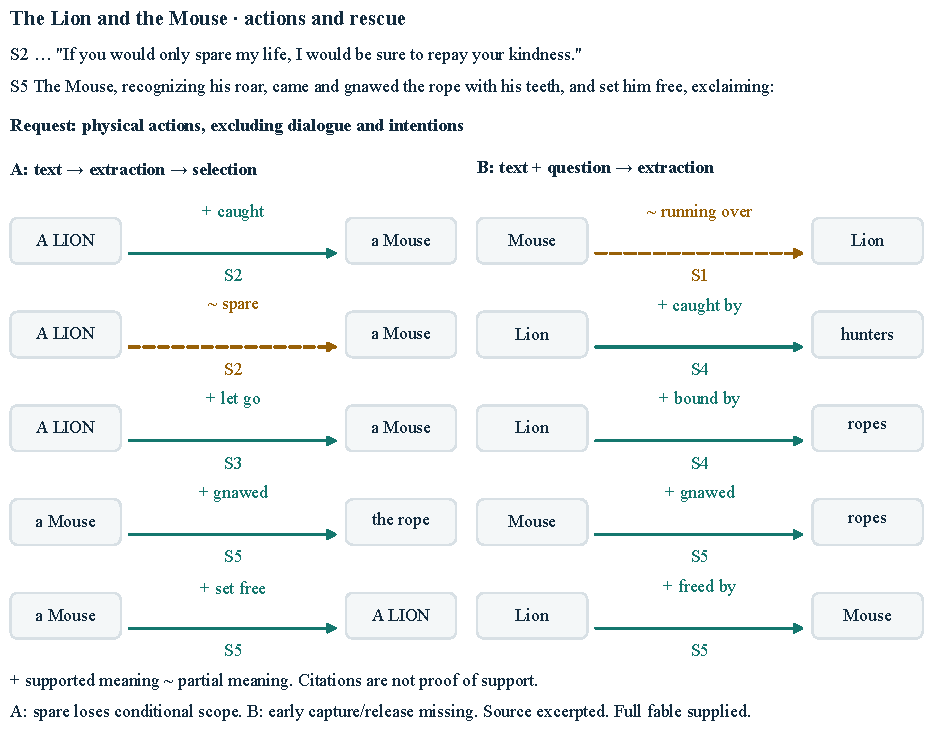
\includegraphics[width=\textwidth,height=.55\textheight,keepaspectratio]{figures/fable.pdf}
\caption{Fable \DIFdelbeginFL \DIFdelFL{actions }\DIFdelendFL \DIFaddbeginFL \DIFaddFL{action records }\DIFaddendFL from \DIFdelbeginFL \DIFdelFL{pre-extract/select }\DIFdelendFL \DIFaddbeginFL \DIFaddFL{fixed selection }\DIFaddendFL (A) and \DIFdelbeginFL \DIFdelFL{independent }\DIFdelendFL contextual extraction (B). + \DIFdelbeginFL \DIFdelFL{indicates }\DIFdelendFL \DIFaddbeginFL \DIFaddFL{marks }\DIFaddendFL supported meaning\DIFdelbeginFL \DIFdelFL{and }\DIFdelendFL \DIFaddbeginFL \DIFaddFL{; }\DIFaddendFL $\sim$ \DIFaddbeginFL \DIFaddFL{marks }\DIFaddendFL partial meaning.\DIFdelbeginFL \DIFdelFL{Display: five of eight A records and all five B records. A's awakening, hunter capture and rope binding are omitted only from display. All predictions remain scored. Executed question: Which physical running/waking, capture, binding, rope-gnawing and release relationships involve the Lion, Mouse, hunters and ropes? Exclude dialogue, intentions, laughter and the moral.\ Source display excerpts S2 and S5 from the complete supplied fable. The spare edge loses conditional scope and retains the misspelled key }\texttt{\DIFdelFL{valid until}}%DIFAUXCMD
\DIFdelFL{. B loses the face-specific running endpoint and omits the early capture/release. Other displayed qualifications are null. Assessments are Codex-authored.}\DIFdelendFL }
\label{fig:fable}
\end{figure*}





\section{EVALUATION}




\subsection{Materials\DIFaddbegin \DIFadd{, Settings }\DIFaddend and \DIFdelbegin \DIFdel{Annotation}\DIFdelend \DIFaddbegin \DIFadd{Reference Answers}\DIFaddend }
\noindent Each \DIFdelbegin \DIFdel{evaluation case combines a numbered narrative $T_i$, a reader's question $q_{ij}$ and reference records $\mathcal{R}_{ij}$, including accepted alternatives:
}\begin{displaymath}
\DIFdel{%DIFDELCMD < \label{eq:evaluation-case}%%%
d_{ij} = \langle T_i, q_{ij}, \mathcal{R}_{ij} \rangle .
}\end{displaymath}%DIFAUXCMD
\DIFdel{Evidence, question scope, reference alternativesand normalization rules are frozen before generation, giving both approaches the same evaluation target}\DIFdelend \DIFaddbegin \DIFadd{case supplies a numbered text, a question and reference answers prepared with Codex before the model runs. These are not a published or independently validated gold standard. ``Accepted alternatives'' are permitted names or relation wordings for the same target, fixed before generation. Both approaches use the same answers and matching rules}\DIFaddend .

\DIFdelbegin \DIFdel{The controlled stories }\DIFdelend Harbor, Orchard and Museum \DIFdelbegin \DIFdel{each contain }\DIFdelend \DIFaddbegin \DIFadd{are short synthetic stories created for this study, each with }\DIFaddend \StorySentences\ evidence sentences. \DIFaddbegin \DIFadd{They are released with their reference answers in the repository. }\DIFaddend Three questions address possession, location within an interval, and belief versus narration\DIFdelbegin \DIFdel{. These tasks reveal whether extracted networks preserve relationships together with their temporal and attribution details}\DIFdelend \DIFaddbegin \DIFadd{, with five, four and four targets respectively}\DIFaddend . Harbor and Orchard informed development. Museum varies sentence order and entity relationships fixed before this batch. Earlier experiments remain separate.

The prose comparison uses Townsend's complete Lion and Mouse fable (\FableWords\ words), the opening of \emph{Alice's Adventures in Wonderland} (\AliceWords\ words), and a contiguous opening passage from \emph{The Red-Headed League} (\HolmesWords\ words) \cite{aesop,carroll,doyle}. Citations identify the retained Gutenberg editions. Passages were selected before execution for identifiable participants, actions, thoughts and dialogue, with two questions per passage addressing actions and claims.

\DIFdelbegin \DIFdel{RelVis demonstrates the value of inspecting extraction errors, while CaRB shows how reference annotations and matching choices affect evaluation }%DIFDELCMD < \cite{schneider2017,bhardwaj2019}%%%
\DIFdel{. Building on these findings, our design connects extraction before or after question disclosure to the preservation of relevance, temporal bounds and attribution in narrative networks. }\DIFdelend \DIFaddbegin \DIFadd{The experiments use }\texttt{\DIFadd{Qwen/Qwen3-8B-AWQ}} \DIFadd{in nonthinking mode }\cite{qwen2025,qwenmodel}\DIFadd{, served by vLLM }\cite{kwon2023} \DIFadd{on one RTX 4090. Temperature is \Temperature, top-p \TopP, top-k \TopK, and seed \Seed. Each response has a \OutputTokens-token limit within a \ContextTokens-token context. We request ordinary JSON without a constrained decoder. The seed records the sampling setup; it does not guarantee identical new responses from the online server. Replaying saved responses reproduces the reported scores without model inference.
}\DIFaddend 

\DIFdelbegin \DIFdel{Synthetic inventories distinguish unsupported relationships from supported but irrelevant ones. Prose }\DIFdelend \DIFaddbegin \DIFadd{The synthetic references enumerate the explicit story facts; prose }\DIFaddend references cover the \DIFdelbegin \DIFdel{requested information. Separate semantic assessments distinguish wording differences from lost or altered meaning . Reference answers and response assessments }\DIFdelend \DIFaddbegin \DIFadd{questions' targets. After generation, Codex assessed the meaning of each output against the supplied text using a rubric fixed before the runs. These assessments and the reference answers }\DIFaddend have not undergone independent human validation. \DIFdelbegin \DIFdel{Ambiguous interpretations, including Holmes 's vocative and Alice 's }\DIFdelend \DIFaddbegin \DIFadd{For example, the Holmes dialogue leaves uncertainty about whom a phrase addresses, while Alice considers whether a }\DIFaddend daisy-chain \DIFdelbegin \DIFdel{consideration, remain open to author review}\DIFdelend \DIFaddbegin \DIFadd{is worthwhile rather than deciding that it is. Such readings are marked unresolved and receive no full semantic-coverage credit.
}

\label{sec:disclosure}
\DIFadd{OpenAI Codex }\cite{openai2025} \DIFadd{also assisted code, figures and manuscript preparation. Qwen produced the experimental relationship records. The semantic assessments are AI-assisted judgments, not independent human ratings}\DIFaddend .




\subsection{Agreement, Meaning and Failure}
\noindent \DIFaddbegin \DIFadd{Evaluation first parses the output, then computes strict matches, and finally reports the separate meaning assessments. }\DIFaddend \emph{Strict qualified-fact matching} requires agreement on the \DIFdelbegin \DIFdel{normalized }\DIFdelend relationship, evidence set, temporal bounds and attribution \DIFaddbegin \DIFadd{after case/whitespace normalization and the listed wording substitutions}\DIFaddend . Let $n$ be the number of predictions, $m$ the number of reference targets and $k$ the number of one-to-one matches against \DIFdelbegin \DIFdel{frozen }\DIFdelend \DIFaddbegin \DIFadd{the prelisted }\DIFaddend alternatives. For nonzero denominators,
\begin{equation}
\label{eq:strict-scores}
P=\frac{k}{n}, \qquad
R=\frac{k}{m}, \qquad
F_1=\frac{2k}{n+m}.
\end{equation}
Incorrect, duplicate, irrelevant and unresolved predictions remain in $n$, while omissions reduce recall. Bare relationship scores ignore citations and qualifications. Strict F1 \DIFdelbegin \DIFdel{therefore measures reference agreement }\DIFdelend \DIFaddbegin \DIFadd{measures agreement with our reference answers}\DIFaddend , not factual truth\DIFaddbegin \DIFadd{: a valid wording absent from the list can fail. The synthetic matcher treats missing nullable fields as unspecified while separately reporting missing keys; the prose matcher requires all eight fields}\DIFaddend .

Semantic assessment \DIFdelbegin \DIFdel{separately labels supported, partially supported, unsupported and unresolved content, alongside qualification }\DIFdelend \DIFaddbegin \DIFadd{labels records as }\emph{\DIFadd{supported}}\DIFadd{, }\emph{\DIFadd{partial}} \DIFadd{(detail or condition lost), }\emph{\DIFadd{unsupported}} \DIFadd{(added or contradicted information), or }\emph{\DIFadd{unresolved}} \DIFadd{(uncertain reading). Time/attribution }\DIFaddend errors and relevance \DIFdelbegin \DIFdel{. Target coverage counts distinct meanings explicitly }\DIFdelend \DIFaddbegin \DIFadd{are recorded separately. Assigning the sister's reading to Alice is unsupported; ``Lion caught by hunters'' preserves meaning despite failing strict wording. Coverage counts distinct reference meanings fully }\DIFaddend preserved. One \DIFdelbegin \DIFdel{prediction may }\DIFdelend \DIFaddbegin \DIFadd{record can }\DIFaddend cover several targets\DIFdelbegin \DIFdel{, but partial support is not full coverage. Support requires positive evidence. Missing meaning is never supplied, and equivalence rules remain unchanged after generation}\DIFdelend \DIFaddbegin \DIFadd{; partial or unresolved meaning receives no full credit. These Codex judgments do not alter strict scores}\DIFaddend .

\DIFdelbegin \DIFdel{Strict parsing rejects malformed JSON , }\DIFdelend \DIFaddbegin \DIFadd{An output is }\emph{\DIFadd{parseable}} \DIFadd{if it is valid JSON with a }\texttt{\DIFadd{facts}} \DIFadd{list, no }\DIFaddend duplicate keys and \DIFaddbegin \DIFadd{no }\DIFaddend non-JSON constants. \DIFdelbegin \DIFdel{A separately recorded recovery may remove }\DIFdelend \DIFaddbegin \DIFadd{This guarantees neither accuracy nor complete record fields. A permitted syntax repair deletes }\DIFaddend only trailing commas \DIFdelbegin \DIFdel{immediately before closing delimiters outside strings, preserving raw bytes and an edit record. Neither main batch required recovery. Unparseable outputs have unavailable graph scores and are not scored as intentionally empty graphs}\DIFdelend \DIFaddbegin \DIFadd{before closing brackets/braces outside quoted text, preserving the original response and deletion positions. Neither batch used this repair. Holmes's two extra-brace failures remain unparseable; their scores are unavailable (NA), not scores for empty answers}\DIFaddend .

\DIFdelbegin \DIFdel{The analysis is descriptive. These purposively selected }\DIFdelend \DIFaddbegin \DIFadd{These }\DIFaddend development examples share stories and reuse outputs\DIFdelbegin \DIFdel{during selection. Records therefore cannot be treated as independent experimental trials, and no significance testsare applied}\DIFdelend \DIFaddbegin \DIFadd{, so records are not independent trials; analysis is descriptive, without significance tests. A follow-up CPU check applies A's unchanged filters to B's saved answers (B+filter), testing selection without new model runs or changes to facts or references}\DIFaddend .

\begin{figure*}[!t]
\centering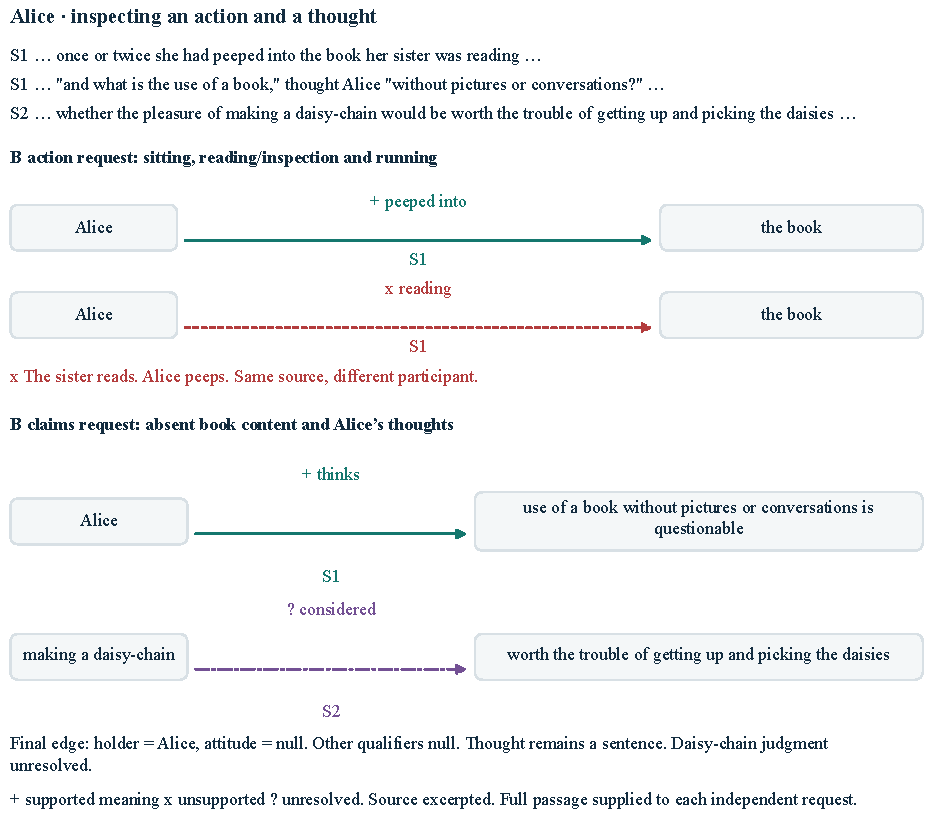
\includegraphics[width=\textwidth,height=.55\textheight,keepaspectratio]{figures/alice.pdf}
\caption{Alice\DIFdelbeginFL \DIFdelFL{: independent contextual extraction (B) for two requests over identical complete evidence. Display: two of five action edges (two sitting edges and Rabbit running omitted) and two of three claims (book content omitted). All remain scored. Executed action question: Which sitting/location, reading/inspection and running relationships involve Alice, her sister, the book, bank and Rabbit? Exclude thoughts, feelings, appearance and book-content properties.\ Executed claims question: What does the passage say about the book's absent content and Alice}\DIFdelendFL 's \DIFdelbeginFL \DIFdelFL{thoughts about the usefulness of such books and making a daisy-chain? Exclude physical actions, locations, appearance and the Rabbit; preserve questions }\DIFdelendFL \DIFaddbeginFL \DIFaddFL{contextual action }\DIFaddendFL and \DIFdelbeginFL \DIFdelFL{consideration without treating them as decisions.\ Source excerpts are marked}\DIFdelendFL \DIFaddbeginFL \DIFaddFL{thought records}\DIFaddendFL . + \DIFdelbeginFL \DIFdelFL{indicates }\DIFdelendFL \DIFaddbeginFL \DIFaddFL{marks }\DIFaddendFL supported meaning, x \DIFdelbeginFL \DIFdelFL{an unsupported }\DIFdelendFL \DIFaddbeginFL \DIFaddFL{a wrong }\DIFaddendFL participant, and ? \DIFaddbeginFL \DIFaddFL{an }\DIFaddendFL unresolved \DIFdelbeginFL \DIFdelFL{consideration. The thought remains the actual sentence-valued object. All bounds are null. The final record has holder Alice and null attitude}\DIFdelendFL \DIFaddbeginFL \DIFaddFL{interpretation}\DIFaddendFL .}
\label{fig:alice}
\end{figure*}






\section{RESULTS}

\subsection{Synthetic Selection and Qualifications}
\noindent All \CompactCalls\ compact-story outputs are strictly parseable. Pre-extract/select (A) matches every possession and dated location target without extras (Table~\ref{tab:compact}). Contextual extraction (B) commonly retrieves the requested physical relationships but returns irrelevant facts in every answer. Orchard's location answer also omits a target: recall is \OrchardLocationRecall. The fresh Museum story shows the same excessive selection as the earlier stories.

\begin{table*}[t]
% Positive inset keeps the top caption within the nominal text margin.
\vspace*{6pt}
\caption{\DIFdelbeginFL \DIFdelFL{Compact-story v2 }\DIFdelendFL \DIFaddbeginFL \DIFaddFL{Synthetic }\DIFaddendFL strict \DIFdelbeginFL \DIFdelFL{qualified-fact scores}\DIFdelendFL \DIFaddbeginFL \DIFaddFL{reference agreement}\DIFaddendFL . A: pre-extract/select\DIFdelbeginFL \DIFdelFL{. }\DIFdelendFL \DIFaddbeginFL \DIFaddFL{; }\DIFaddendFL B: contextual extraction\DIFaddbeginFL \DIFaddFL{; B+f: B with the unchanged fixed filters}\DIFaddendFL . $n$ \DIFdelbeginFL \DIFdelFL{includes every prediction. Targets per story: possession 5, location 4, belief/reality 4. No historical recoveries are pooled}\DIFdelendFL \DIFaddbeginFL \DIFaddFL{counts all predictions}\DIFaddendFL .}\label{tab:compact}
\centering\small\DIFdelbeginFL %DIFDELCMD < \begin{tabular}{llrrrrrrrr}%%%
\DIFdelendFL \DIFaddbeginFL \setlength{\tabcolsep}{4pt}
\begin{tabular}{llrrrrrrrrr}\DIFaddendFL \toprule
Story & Question & $n_A$ & $P_A$ & $R_A$ & $F1_A$ & $n_B$ & $P_B$ & $R_B$ & $F1_B$ \DIFaddbeginFL & \DIFaddFL{$F1_{B+f}$}\DIFaddendFL \\\midrule
Harbor & Possession & 5 & 1.000 & 1.000 & 1.000 & 10 & 0.500 & 1.000 & 0.667 \DIFaddbeginFL & \DIFaddFL{1.000 }\DIFaddendFL \\
Harbor & Location & 4 & 1.000 & 1.000 & 1.000 & 6 & 0.667 & 1.000 & 0.800 \DIFaddbeginFL & \DIFaddFL{1.000 }\DIFaddendFL \\
Harbor & Belief/reality & 5 & 0.000 & 0.000 & 0.000 & 14 & 0.143 & 0.500 & 0.222 \DIFaddbeginFL & \DIFaddFL{0.000 }\DIFaddendFL \\
Orchard & Possession & 5 & 1.000 & 1.000 & 1.000 & 12 & 0.417 & 1.000 & 0.588 \DIFaddbeginFL & \DIFaddFL{1.000 }\DIFaddendFL \\
Orchard & Location & 4 & 1.000 & 1.000 & 1.000 & 5 & 0.600 & 0.750 & 0.667 \DIFaddbeginFL & \DIFaddFL{0.857 }\DIFaddendFL \\
Orchard & Belief/reality & 4 & 1.000 & 1.000 & 1.000 & 13 & 0.154 & 0.500 & 0.235 \DIFaddbeginFL & \DIFaddFL{0.000 }\DIFaddendFL \\
Museum & Possession & 5 & 1.000 & 1.000 & 1.000 & 13 & 0.385 & 1.000 & 0.556 \DIFaddbeginFL & \DIFaddFL{1.000 }\DIFaddendFL \\
Museum & Location & 4 & 1.000 & 1.000 & 1.000 & 5 & 0.800 & 1.000 & 0.889 \DIFaddbeginFL & \DIFaddFL{1.000 }\DIFaddendFL \\
Museum & Belief/reality & 4 & 0.000 & 0.000 & 0.000 & 14 & 0.143 & 0.500 & 0.222 \DIFaddbeginFL & \DIFaddFL{0.000 }\DIFaddendFL \\\bottomrule\end{tabular}\end{table*}


Orchard\DIFdelbegin \DIFdel{illustrates actual selection from a broader model extraction (Figure~\ref{fig:orchard}). Its five }\DIFdelend \DIFaddbegin \DIFadd{'s five selected }\DIFaddend ownership/carrying records connect six nodes \DIFdelbegin \DIFdel{, retaining explicit carrying intervals . This illustration does not establish a construction effect}\DIFdelend \DIFaddbegin \DIFadd{and retain explicit intervals (Figure~\ref{fig:orchard})}\DIFaddend . The companion contrasts this \DIFdelbegin \DIFdel{slice with the }\DIFdelend \DIFaddbegin \DIFadd{selection with B's }\DIFaddend twelve-record \DIFdelbegin \DIFdel{contextual answer, which also retains }\DIFdelend \DIFaddbegin \DIFadd{answer, containing }\DIFaddend seven irrelevant locations. \DIFaddbegin \DIFadd{This illustrates selection, not a new ontology-construction capability.
}\DIFaddend 

Among emitted records with identifiable explicitly timed sources, \IntervalsKept\ of \IntervalsEligible\ preserve their full intervals, including irrelevant records. This is conditional preservation, not temporal recall over every reference. The companion's Harbor timeline distinguishes these intervals from the query window. Attribution is less stable: Orchard's pre-extraction decomposes beliefs correctly, whereas Harbor and Museum use sentence-valued belief objects that disrupt selection.

\DIFaddbegin \DIFadd{Applying the same fixed filters to the contextual answers checks the role of selection (B+f in Table~\ref{tab:compact}). All possession targets and the Harbor/Museum location targets match without extras. Orchard location F1 rises to 0.857, but its missing fact remains missing. Belief/reality F1 falls to zero in all three stories: the filters cannot recover the intended objects from sentence-valued beliefs and discard needed narrated locations. Across the five parseable contextual prose answers, strict F1 is unchanged; the fable claims answer loses one record. The Holmes failures remain unavailable.
}




\DIFaddend \subsection{Published Prose and Partial Meaning}
\noindent The prose comparison yields \ProseParsed\ strictly parseable responses from \ProseCalls\ calls. Extra closing braces invalidate Holmes's pre-extraction and contextual action answer. The shared pre-extraction failure blocks both A questions (Table~\ref{tab:prose}). The parseable Holmes claims answer contains partial and unresolved content without fully covered targets.

\begin{table*}[t]
\vspace*{6pt}
\caption{Published prose: strict agreement and \DIFdelbeginFL \DIFdelFL{Codex-authored }\DIFdelendFL \DIFaddbeginFL \DIFaddFL{Codex }\DIFaddendFL semantic \DIFdelbeginFL \DIFdelFL{assessment. A: pre-extract/select. B: contextual extraction}\DIFdelendFL \DIFaddbeginFL \DIFaddFL{assessments}\DIFaddendFL . S/P/X/U\DIFdelbeginFL \DIFdelFL{counts }\DIFdelendFL \DIFaddbeginFL \DIFaddFL{: }\DIFaddendFL supported\DIFdelbeginFL \DIFdelFL{, }\DIFdelendFL \DIFaddbeginFL \DIFaddFL{/}\DIFaddendFL partial\DIFdelbeginFL \DIFdelFL{, }\DIFdelendFL \DIFaddbeginFL \DIFaddFL{/}\DIFaddendFL unsupported\DIFdelbeginFL \DIFdelFL{and }\DIFdelendFL \DIFaddbeginFL \DIFaddFL{/}\DIFaddendFL unresolved records\DIFdelbeginFL \DIFdelFL{. Coverage counts preserved target meanings. }\DIFdelendFL \DIFaddbeginFL \DIFaddFL{; }\DIFaddendFL NA\DIFdelbeginFL \DIFdelFL{denotes }\DIFdelendFL \DIFaddbeginFL \DIFaddFL{: }\DIFaddendFL parse failure\DIFdelbeginFL \DIFdelFL{, not an empty graph. All parseable predictions cite valid evidence IDs, which does not establish support}\DIFdelendFL .}\label{tab:prose}
\centering\small\begin{tabular}{lllrrrrrr}\toprule
Passage & Question & Method & $n$ & Precision & Recall & F1 & S/P/X/U & Coverage\\\midrule
Alice & Actions & A & 2 & 0.500 & 0.200 & 0.286 & 2/0/0/0 & 3/5 \\
Alice & Actions & B & 5 & 0.400 & 0.400 & 0.400 & 3/1/1/0 & 3/5 \\
Alice & Claims & A & 4 & 0.000 & 0.000 & 0.000 & 2/2/0/0 & 1/4 \\
Alice & Claims & B & 3 & 0.000 & 0.000 & 0.000 & 2/0/0/1 & 3/4 \\
Fable & Actions & A & 8 & 0.625 & 0.625 & 0.625 & 6/1/0/1 & 6/8 \\
Fable & Actions & B & 5 & 0.400 & 0.250 & 0.308 & 4/1/0/0 & 4/8 \\
Fable & Claims & A & 1 & 0.000 & 0.000 & 0.000 & 1/0/0/0 & 2/5 \\
Fable & Claims & B & 4 & 0.000 & 0.000 & 0.000 & 1/3/0/0 & 0/5 \\
Holmes & Actions & A & NA & NA & NA & NA & NA & NA \\
Holmes & Actions & B & NA & NA & NA & NA & NA & NA \\
Holmes & Claims & A & NA & NA & NA & NA & NA & NA \\
Holmes & Claims & B & 3 & 0.000 & 0.000 & 0.000 & 0/1/0/2 & 0/5 \\\bottomrule\end{tabular}\end{table*}


For fable actions, pre-extract/select performs better on both measures, with strict F1 \FableAFone\ versus \FableBFone\ and semantic coverage \FableACoverage\ versus \FableBCoverage. A therefore preserves most target action meanings. Both approaches recover the later rescue, but contextual extraction omits the early capture and release. A's \texttt{spare} relation loses the scope of the Mouse's conditional plea, while some supported passive formulations fail strict matching (Figure~\ref{fig:fable}). These networks capture useful narrative content despite incomplete agreement.

In the Alice excerpt, contextual extraction improves semantic coverage from \AliceACoverage\ to \AliceBCoverage, although both strict F1 scores remain zero. Its combined thought statement preserves rhetorical meaning without the requested decomposition. Contextual extraction also incorrectly assigns reading to Alice instead of her sister. Whether the daisy-chain record converts considering an action's worth into judging it worthwhile remains unresolved (Figure~\ref{fig:alice}). The improvement is therefore in retained meaning, with participant errors and interpretive uncertainty still visible.









\section{DISCUSSION AND LIMITATIONS}

\noindent \DIFdelbegin \DIFdel{This work advances narrative ontology development through an implemented model connecting reader intent, temporal scope and evidence inspection. It makes the construction of a narrative network an explicit part of answering a question, with relationships represented together with the information needed to interpret and verify them.
Building on relation extraction }%DIFDELCMD < \cite{banko2007}%%%
\DIFdel{, temporal and perspective representation }%DIFDELCMD < \cite{time2017,fokkens2017}%%%
\DIFdel{, and visual error analysis }%DIFDELCMD < \cite{schneider2017}%%%
\DIFdel{, the contribution is a shared framework for comparing how questionavailability affects extraction and selection. Relevance and interval filters provide a mechanism for reducing displayed graph size while retaining source evidence and original temporal bounds. Contextual generation explores the complementary possibility of focusing relationships during extraction itself}\DIFdelend \DIFaddbegin \DIFadd{A reuses one extraction for several questions and works well with these specific filters, but cannot recover facts omitted during extraction. B can express relationships tailored to a question, as in Alice's thoughts, but often returns extra facts and requires another model call per question. B+filter removes some extras; missing facts and poorly structured beliefs remain problems}\DIFaddend .

The \DIFdelbegin \DIFdel{examples demonstrate useful preservation of narrative structure. Pre-extraction captures most annotated fable actions, contextual extraction increases semantic coverage in Alice, and Harbor retains explicit intervals. These findings establish concrete capabilities on which further ontology development can build. The framework also connects participant errors, lost conditions and irrelevant relationships to their source passages, making improvements in parsing and selection directly assessable. Its value lies in combining usable partial networks with an explicit account of what they preserve and omit}\DIFdelend \DIFaddbegin \DIFadd{records guarantee neither completeness nor logical consistency. Parsing checks syntax and matching checks specified targets, not all possible facts. Identity uses local names, beliefs may conflict with narration, and numeric bounds omit relative narrative time. Evidence covers six short texts, one model and one seed, with passage-specific filters and Codex-authored references and assessments. No independent annotation study, external-system comparison or usability evaluation was conducted. Reusing these outputs for the filter check adds no evidence about generalization. Longer unseen passages, independent annotators and repeated runs are needed to test whether either method is generally better}\DIFaddend .




\section{CONCLUSION}
\noindent \DIFdelbegin \DIFdel{We present a workflow connecting narrative questions, qualified relationships and evidence inspection. Comparing pre-extract}\DIFdelend \DIFaddbegin \DIFadd{Pre-extract}\DIFaddend /select \DIFdelbegin \DIFdel{with contextual extraction reveals useful action and thought information alongside relevance and participant errors. Selection performs better on several questions, while contextual }\DIFdelend \DIFaddbegin \DIFadd{gives cleaner possession and location answers and preserves more fable actions in these examples. Contextual }\DIFaddend extraction preserves more of Alice's \DIFdelbegin \DIFdel{claims. Combining strict agreement, semantic assessment and visualization provides a concrete basis for improving narrative extraction and studying its use.
}%DIFDELCMD < 

%DIFDELCMD < %%%
\section{\DIFdel{AI USE AND ANNOTATION PROVENANCE}}
%DIFAUXCMD
\addtocounter{section}{-1}%DIFAUXCMD
%DIFDELCMD < \label{sec:disclosure}
%DIFDELCMD < \noindent %%%
\DIFdel{OpenAI Codex }%DIFDELCMD < \cite{openai2025} %%%
\DIFdel{assisted implementation of code. Qwen generated the simulated user prompt exchange for query ontological searches}\DIFdelend \DIFaddbegin \DIFadd{thought content but assigns reading to the wrong person. Fixed filters remove some extra facts without recovering omissions. Next steps are independent annotation review, longer unseen passages and comparison with other extraction systems, including ATOM}\DIFaddend .


{\small\begin{thebibliography}{}

\bibitem[{Aesop}, 2008]{aesop}
{Aesop} (2008).
\newblock {\em Three Hundred {Aesop's} Fables}.
\newblock Project Gutenberg, ebook 21.
\newblock G. F. Townsend, trans. Digital edition released 25 June 2008, updated
  15 October 2025. Retrieved 9 September 2026.
  \url{https://www.gutenberg.org/ebooks/21}.

\bibitem[Banko et~al., 2007]{banko2007}
Banko, M., Cafarella, M.~J., Soderland, S., Broadhead, M., and Etzioni, O.
  (2007).
\newblock Open information extraction from the web.
\newblock In {\em Proceedings of the 20th International Joint Conference on
  Artificial Intelligence (IJCAI)}, pages 2670--2676.

\bibitem[Bhardwaj et~al., 2019]{bhardwaj2019}
Bhardwaj, S., Aggarwal, S., and {Mausam} (2019).
\newblock {CaRB}: A crowdsourced benchmark for open {IE}.
\newblock In {\em Proceedings of {EMNLP-IJCNLP}}, pages 6262--6267. Association
  for Computational Linguistics.
\newblock \url{https://doi.org/10.18653/v1/D19-1651}.

\bibitem[Carroll, 2008]{carroll}
Carroll, L. (2008).
\newblock {\em Alice's Adventures in Wonderland}.
\newblock Project Gutenberg, ebook 11.
\newblock Digital edition released 27 June 2008, updated 26 June 2025. Chapter
  I. Retrieved 9 September 2026. \url{https://www.gutenberg.org/ebooks/11}.

\bibitem[Caufield et~al., 2024]{caufield2024}
Caufield, J.~H., Hegde, H., Emonet, V., Harris, N.~L., Joachimiak, M.~P.,
  Matentzoglu, N., Kim, H., Moxon, S., Reese, J.~T., Haendel, M.~A., Robinson,
  P.~N., and Mungall, C.~J. (2024).
\newblock Structured prompt interrogation and recursive extraction of semantics
  ({SPIRES}): a method for populating knowledge bases using zero-shot learning.
\newblock {\em Bioinformatics}, 40(3):btae104.
\newblock \url{https://doi.org/10.1093/bioinformatics/btae104}.

\bibitem[Cox and Little, 2017]{time2017}
Cox, S. and Little, C., editors (2017).
\newblock {\em Time Ontology in {OWL}}.
\newblock World Wide Web Consortium.
\newblock W3C Recommendation, 19 October 2017.
  \url{https://www.w3.org/TR/2017/REC-owl-time-20171019/}.

\bibitem[Doyle, 1999]{doyle}
Doyle, A.~C. (1999).
\newblock {\em The Adventures of Sherlock Holmes}.
\newblock Project Gutenberg, ebook 1661.
\newblock Digital edition released 1 March 1999, updated 10 October 2023. The
  Red-Headed League. Retrieved 9 September 2026.
  \url{https://www.gutenberg.org/ebooks/1661}.

\DIFaddbegin \bibitem[Fader et~al., 2011]{fader2011}
\DIFadd{Fader, A., Soderland, S., and Etzioni, O. (2011).
}\newblock \DIFadd{Identifying relations for open information extraction.
}\newblock \DIFadd{In }{\em \DIFadd{Proceedings of EMNLP}}\DIFadd{, pages 1535--1545. Association for
  Computational Linguistics.
}

\DIFaddend \bibitem[Fokkens et~al., 2017]{fokkens2017}
Fokkens, A., Vossen, P., Rospocher, M., Hoekstra, R., and van Hage, W.~R.
  (2017).
\newblock {GRaSP}: Grounded representation and source perspective.
\newblock In {\em Proceedings of the Workshop Knowledge Resources for the
  Socio-Economic Sciences and Humanities associated with {RANLP} 2017}, pages
  19--25. INCOMA Inc.
\newblock \url{https://doi.org/10.26615/978-954-452-040-3_003}.

\bibitem[Heer and Shneiderman, 2012]{heer2012}
Heer, J. and Shneiderman, B. (2012).
\newblock Interactive dynamics for visual analysis.
\newblock {\em Communications of the ACM}, 55(4):45--54.
\newblock \url{https://doi.org/10.1145/2133416.2146416}.

\bibitem[Kwon et~al., 2023]{kwon2023}
Kwon, W., Li, Z., Zhuang, S., Sheng, Y., Zheng, L., Yu, C.~H., Gonzalez, J.~E.,
  Zhang, H., and Stoica, I. (2023).
\newblock Efficient memory management for large language model serving with
  {PagedAttention}.
\newblock In {\em Proceedings of the 29th Symposium on Operating Systems
  Principles (SOSP)}, pages 611--626. Association for Computing Machinery.
\newblock \url{https://doi.org/10.1145/3600006.3613165}.

\DIFaddbegin \bibitem[Lairgi et~al., 2026]{lairgi2026}
\DIFadd{Lairgi, Y., Moncla, L., Benabdeslem, K., Cazabet, R., and Cl}{\DIFadd{\'e}}\DIFadd{au, P. (2026).
}\newblock {\DIFadd{ATOM}}\DIFadd{: }{\DIFadd{AdapTive}} \DIFadd{and }{\DIFadd{OptiMized}} \DIFadd{dynamic temporal knowledge graph
  construction using }{\DIFadd{LLMs}}\DIFadd{.
}\newblock \DIFadd{In }{\em \DIFadd{Findings of the Association for Computational Linguistics:
  EACL 2026}}\DIFadd{, pages 950--966. Association for Computational Linguistics.
}

\bibitem[{Mausam} et~al., 2012]{mausam2012}
{\DIFadd{Mausam}}\DIFadd{, Schmitz, M., Soderland, S., Bart, R., and Etzioni, O. (2012).
}\newblock \DIFadd{Open language learning for information extraction.
}\newblock \DIFadd{In }{\em \DIFadd{Proceedings of EMNLP-CoNLL}}\DIFadd{, pages 523--534. Association for
  Computational Linguistics.
}

\DIFaddend \bibitem[{OpenAI}, 2025]{openai2025}
{OpenAI} (2025).
\newblock Introducing {Codex}.
\newblock \url{https://openai.com/index/introducing-codex/}.
\newblock 16 May. Tool announcement.

\bibitem[{Qwen Team}, nd]{qwenmodel}
{Qwen Team} (n.d.).
\newblock {Qwen3-8B-AWQ} model card and pinned snapshot.
\newblock
  \href{https://huggingface.co/Qwen/Qwen3-8B-AWQ/tree/4da05a8edb55c6046cce958586c33b61da07bb79}{Hugging
  Face, pinned snapshot}.
\newblock Revision specified in appendix. Accessed 9 September 2026.

\bibitem[Schneider et~al., 2017]{schneider2017}
Schneider, R., Oberhauser, T., Klatt, T., Gers, F.~A., and L{\"o}ser, A.
  (2017).
\newblock Analysing errors of open information extraction systems.
\newblock In {\em Proceedings of the First Workshop on Building Linguistically
  Generalizable {NLP} Systems}, pages 11--18. Association for Computational
  Linguistics.
\newblock \url{https://doi.org/10.18653/v1/W17-5402}.

\bibitem[Yang et~al., 2025]{qwen2025}
Yang, A., Li, A., Yang, B., et~al. (2025).
\newblock {Qwen3} technical report.
\newblock arXiv:2505.09388.

\end{thebibliography}
}
\section*{APPENDIX}
\noindent \DIFaddbegin \DIFadd{Code, exact requests, outputs, reference answers and companion: }\url{https://github.com/mantzaris/StoryProjectionOnto}\DIFadd{, under }\path{paper/icaart2027/}\DIFadd{; the revision README gives CPU replay instructions. }\DIFaddend Qwen3-8B-AWQ revision: \texttt{4da05a8edb55c6046cce9585}\allowbreak\texttt{86c33b61da07bb79}. Software: vLLM 0.10.2, Transformers 4.55.2\DIFdelbegin \DIFdel{. The pinned templateuses }\DIFdelend \DIFaddbegin \DIFadd{; template: }\DIFaddend \texttt{enable\_thinking=False}\DIFdelbegin \DIFdel{. The concise companion indexes complete machine-readable requests, outputs, reference alternatives and assessments}\DIFdelend .
\end{document}
